%!TEX root = ../Main.tex

\chapter{Unsupervised learning and principal components}

When we are talking about unsupervised learning, we are talking about the problem of creating machine learning, without access to labeled data. With unlabeled data we can’t make predictions of a response which often is the case with supervised learning. Instead we can try to group data based on features of the dataset at try to make assumptions based on this.

PCA is a way of doing just that, as well as other things. Principal component analysis let us investigate data even with a very high dimensional feature set. Under normal circumstances we would not be able to illustrate the more than two or maybe three features of a data set. So how do we cluster the data points together if can’t evaluate more than two or three features. We use Principal component analysis. 

PCA works by trying to investigate how much information is stored within each feature about the datapoints. With PCA we create different principal components, based on the number of features. The first principal component would be the linear combination of the features which maximizes the datapoints distance to the origin of the plot. This value could also be the variance. When this linear combination is found we find the next one by determining the linear combination that goes through the origin and is perpendicular to the first one. This is done for every feature in the dataset.

When all the principal components are calculated and maybe illustrated, we can calculate which of the principal components, contributes most to the diversion between the samples. The two components which has the highest contribution is chosen for the 2D PCA plot. We calculate the contribution by looking at the sum of the squared distances from the datapoints to the principal component. The sum of squared distances from a single component, held against the entire dataset would yield how much contribution to the variation in the set that each component has.

\begin{figure}[H]
	\centering
	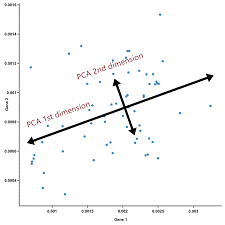
\includegraphics[width=\textwidth]{Img/pca.PNG}
	\caption{PCA plot of two principal components}
	\label{fig:pca_plot}
\end{figure}  

Therefore, when we are choosing two different components for the PCA plot, the first component will have a higher say in the difference between the data points in that direction. From the picture seen above at figure \ref{fig:pca_plot} we can conclude that the datapoints that are separated in the X direction is more different than the datapoints that are divided in the Y direction. The higher the contribution from both the chosen components are, the better a representation of the dataset, the plot will present. 



